% !TEX TS-program = pdflatex
% !TEX encoding = UTF-8 Unicode

% This is a simple template for a LaTeX document using the "article" class.
% See "book", "report", "letter" for other types of document.

\documentclass[11pt]{article} % use larger type; default would be 10pt

%\usepackage[utf8]{inputenc} % set input encoding (not needed with XeLaTeX)


%%% Examples of Article customizations
% These packages are optional, depending whether you want the features they provide.
% See the LaTeX Companion or other references for full information.

%%% PAGE DIMENSIONS
\usepackage{geometry} % to change the page dimensions
\geometry{a4paper} % or letterpaper (US) ocher a5paper or....
\geometry{margin=1in} % for example, change the margins to 2 inches all round
% \geometry{landscape} % set up the page for landscape
%   read geometry.pdf for detailed page layout information
\usepackage{graphicx} 
% \usepackage[parfill]{parskip} % Activate to begin paragraphs with an empty line rather than an indent

%%% PACKAGES
%\usepackage{booktabs} % for much better looking tables
\usepackage{array} % for better arrays (eg matrices) in maths
%\usepackage{paralist} % very flexible & customisable lists (eg. enumerate/itemize, etc.)
\usepackage{verbatim} % adds environment for commenting out blocks of text & for better verbatim
%\usepackage{subfig} % make it possible to include more than one captioned figure/table in a single float
% These packages are all incorporated in the memoir class to one degree or another...

%%% HEADERS & FOOTERS
\usepackage{fancyhdr} % This should be set AFTER setting up the page geometry
\pagestyle{fancy} % options: empty , plain , fancy
\renewcommand{\headrulewidth}{0pt} % customise the layout...
\lhead{}\chead{}\rhead{}
\lfoot{}\cfoot{\thepage}\rfoot{}

%%% SECTION TITLE APPEARANCE
%\usepackage{sectsty}
%\allsectionsfont{\sffamily\mdseries\upshape} % (See the fntguide.pdf for font help)
% (This matches ConTeXt defaults)

%%% ToC (table of contents) APPEARANCE
%\usepackage[nottoc,notlof,notlot]{tocbibind} % Put the bibliography in the ToC
%\usepackage[titles,subfigure]{tocloft} % Alter the style of the Table of Contents
%\renewcommand{\cftsecfont}{\rmfamily\mdseries\upshape}
%\renewcommand{\cftsecpagefont}{\rmfamily\mdseries\upshape} % No bold!

%\usepackage[T1]{fontenc}
\usepackage[latin9]{inputenc}
%\usepackage[active]{srcltx}
\usepackage{setspace}
\usepackage{lscape}
\doublespacing
\usepackage[english]{babel}
\bibliographystyle{plain}



\begin{document}

\title{Approaches for Large Scale Metagenome Assembly}
\author{ACH, JMT, CTB}
\maketitle

\section{Introduction}  
Complex microbial communities operate at the heart of many crucial environmental, ecological, and biomedical processes, providing critical ecosystem functionality that underpins all of biology (\cite{Arumugam:2011p735,Hess:2011p686,Iverson:2012p1281,Mackelprang:2011p1087,Qin:2010p189,Tringe:2005p174,Venter:2004p170}).  These systems are difficult to study in situ, and consequently, we lack a fundamental understanding of their diversity and function, much less how they self-assemble, maintain themselves, and evolve through time.  Advances in DNA sequencing technologies now provide unprecedented access to these communities in the form of millions to billions of short-read sequences of environmental DNA  \cite{Hess:2011p686,Mackelprang:2011p1087,Qin:2010p189}.   Even more sequencing is needed to detect the rare species in environmental samples, e.g., up to 50 Tbp for an individual gram of soil \cite{Gans:2005p1365}.   Both the read lengths and scale of sequencing data pose new challenges to traditional analysis approaches of sequencing data.  Short read lengths and their associated sequencing errors and biases have little biological signal and are noisy, limiting direct annotation approaches against known reference genomes.  Further complicating analysis is the majority of genes sequenced from metagenomes are not similar to known genes \cite{Arumugam:2011p735,Qin:2010p189}.  

\emph{De novo} assembly of raw sequencing data offers several advantages to metagenomic sequencing datasets.  It significantly reduces the total number of sequences for analysis by identifying consensus sequences from overlapping reads.  The assembled contigs are longer than sequencing reads and provide gene order.  Importantly, \emph{de novo} assembly does not rely on the existence of reference genomes, allowing the discovery of novel elements.   The main challenge for metagenomic applications of \emph{do novo} assembly is that current assembly tools do not scale to the volumes of metagenomic datasets being generated. Assembled metagenomes from the rumen, human gut, and permafrost soils required processing of only the most abundant sequences  \cite{Hess:2011p686,Mackelprang:2011p1087,Qin:2010p189}.  Traditional assemblers have been designed for the assembly of single genomes whose abundance distribution and diversity content are significantly different from the mixed populations of metagenomes.  Although many new metagenome-specific assemblers have been developed to address characteristics of mixed population assembly, these are limited to sample diversity and volume.    

In this study, we present a set of approaches which enable large-scale metagenomic de novo assembly.  We initially reduce the dataset volume by normalizing sequencing coverage and removing sequencing errors and biases.  We subsequently partition reads based on biological connectivity, resulting in partitions which can be assembled with significantly reduced computational requirements.   Using a human gut mock community dataset, we demonstrate that our approaches at reducing and partitioning datasets are effective at producing nearly identical assemblies and consequently extend our approaches to two of the largest published soil metagenomes which have previously been impossible to assemble. 

\section{Results}

\subsection{Case study:  Assembly of mock metagenome}

\subsubsection{Evaluation of data reduction through digital normalization and high abundance filtering}

Using the described approaches (see Methods and Supp Info), a total of 5.9 million reads (40\% of total reads) were removed from a human gut community mock dataset.   We compared the presence of reference genomes known to be present within the mock dataset  in the original and filtered sequencing reads.  Specifically, the representation of reference genomes by sequencing reads and the ability to recover these reference genomes after assembly were evaluated.   The abundance of reference genomes was estimated based on the coverage of sequencing reads in the original dataset, and a total of 30 reference genomes were estimated to have been sequenced to a coverage of greater than 3-fold, ranging from 6-fold to 2,000-fold coverages (Table ~\ref{referencestats} and Figures ~\ref{coverage1} and ~\ref{coverage2}).  Overall, a total of 91\% of the available reference genomes were covered by the reads in the original dataset.  After digital normalization and high abundance filtering, the remaining sequencing reads covered a total of 93\% of the available reference genomes.   After assembly (Velvet), the recovery of reference genomes by the contigs assembled from the original and filtered datasets were compared, resulting in recoveries of 43\% and 44\% of references, respectively.  The assembly of the original dataset contained 29,063 contigs and 38 million bp compared to the filtered assembly containing 30,082 contigs and 35 million bp (Table ~\ref{assemblystats}).  Comparable recoveries of references between original and filtered datasets were also obtained for other assemblers (SOAPdenovo and Meta-IDBA).   Overall, the genomic content of both assemblies were similar to one another, ~94\%, and furthermore, the filtered and filtered / partitioned assemblies were greater than 99\% identical to each other.  For the filtered dataset, the time and memory requirements for de novo assembly were significantly reduced.  Specifically, the data reduction took less than four hours, and the time and memory for assembly (Velvet) was reduced from 12 GB and 4 hours for the unfiltered dataset to 3 GB and less than an hour for the filtered dataset.   

The abundance of assembled contigs and reference genomes was estimated by the sequencing coverage of reads (Figures ~\ref{diginormreference} and ~\ref{coveragecompare}).   It was found that above a sequencing coverage of five, the majority of reads which could be mapped to reference genomes were also included in an assembled contig (Figure ~\ref{coveragehmp}).  Below this threshold, reads could be mapped to reference genomes but were less likely to be associated with assembled contigs in either the unfiltered or filtered assemblies.   Assembled contigs from the original dataset and filtered datasets were used to estimate the abundance of 
genomes present within the dataset.  Using a one-directional, paired t-test of squared deviations, the difference between the estimated abundances of the original and filtered assembled contigs were compared against those of the associated reference genomes.  As we expected the filtered assembly to have increased accuracy due to a reduction of errors, we used a one-sided t-test and found that abundance estimations from the filtered assembly were significantly closer to predicted abundances from reference genomes (p-value of 0.032).  

\subsubsection{Evaluation of partitioning reads based on connectivity}
For the 9 million reads in the filtered dataset, we identified a total of 85,818 partitions containing a minimum of five reads and among these, only 2,359 partitions contained reads originating from more than one genome.  With the exception of one partition containing reads from 36 reference chromosomes and/or plasmids, all other partitions contained reads from less than nine genomes.  The number of partitions associated with reads which were associated with reference genomes were examined and, in general, reference genomes with high coverage had fewer partitions (Table ~\ref{referencestats}).  There were 112 partitions associated with high abundance reference genomes (coverage above 25) compared to 2,771 partitions associated with low abundance genomes (coverage below 25).  In the case of multiple partitions associated with a low abundance genome, reads aligning to similar regions of a reference genome were associated with a the same partition (SI Figure ~\ref{partitionreference}).

To further evaluate our approaches, spiked reads (containing errors) from known reference genomes were introduced to the mock community dataset and the recovery of these references were evaluated.  Initially, a single  spiked reference genome (E. coli strain E24377A, NC\_009801.1) was added to the  a ``spiked" mock community dataset and processed identically to the original mock dataset.  This resulted in similar amounts of data reduction after digital normalization and partitioning (Table ~\ref{referencestats}).  Among the 81,154 partitioned sets of reads, we identified only 2,580 partitions containing reads from multiple genomes.  A total of 424 partitions contained reads from the spiked E. coli genome, among these 201 partitions contained \emph{only} spiked reads (Figure ~\ref{ecolimap}).  The assembly of these 424 partitions resulted in contigs which when aligned against the E. coli strain E24377A genome overlapped 99.5\% (4957067 of 4979619 bp) of the original reference.  Next, a similar analysis introducing five closely-related spiked E. coli strains into the mock community dataset was  performed.  Partitioning this ``mix-spiked" mock community dataset resulted in 81,425 partitions, of which only 1,154 partitions contained reads associated with multiple genomes.  Among the partitions which contained reads associated with a single genome, 658 partitions contained reads originating from one of the spiked E. coli strains.  In partitions containing greater than one genome, 224 partitions contained reads from a spiked E. coli strain and either another spiked strain or from the mock community dataset (Figure ~\ref{ecolimap}).  The partitions containing any reads originating from the spiked E. coli strains were identified and assembled independently.  Among the resulting 6,076 contigs, all but three contigs could be identified as originating from a spiked E. coli genome (e.g., top blast hit).  The remaining three contigs were greater than 99\% similar to HMP mock reference genomes (NC\_000915.1, NC\_003112.2, and NC\_009614.1).  The contigs associated with E. Coli were aligned against the spiked reference genomes, recovering greater than 98\% of each of the five genomes.  Many of these contigs were associated with reads originating from multiple genomes (Figure ~\ref{fractionassembled}), 3,075 contigs (51\%) contained reads which were mapped from more than one spiked genome.  This result is comparable to the fraction of contigs which are associated with multiple genomes when the original (unfiltered) dataset is assembled, resulting in 4,702 contigs associated with the ``spiked reads", of which 66\% contained reads originating from more than one spiked genome.

\subsection{Characteristics of soil metagenomes}

Our approaches were extended to the de novo assembly of two soil metagenomes.  Previously, the assembly of the Iowa corn and prairie datasets containing 1.8 billion and 3.3 billion reads, respectively, were impossible in 500 GB of memory.   A 75 million reads subset of the Iowa corn dataset alone required 110 GB of memory (Figure ~\ref{memory}).  Applying the same filtering approaches as applied to the HMP mock dataset, the Iowa corn and prairie datasets were reduced to 1.4 million and 2.2 million reads, respectively, and after partitioning, a total of 1.0 million and 1.7 million reads remained, respectively.  Notably, the Iowa corn and prairie were sampled at significantly lower sequencing coverages than the mock community dataset.  Whereas has the mock dataset had only 33\% of its k-mers (k=20) present less than ten-times in the dataset, the Iowa corn and prairie datasets contained 53\% and 43\%, respectively, of all k-mers with less than ten-fold coverage.  The large majority of k-mers in the soil metagenomes are relatively low-coverage (Figure ~\ref{diginormcoverage}), and consequently, digital normalization did not remove as many reads in the soil metagenomes.

\subsubsection{Assembly of soil metagenomes}

Based on the mock community dataset, we estimated that above a sequencing depth of 6, the large majority of sequences could be assembled (Figure ~\ref{coveragehmp}).  Given the greater diversity expected in the soil metagenomes, we normalized these datasets to a coverage threshold of 20.  After partitioning the filtered datasets, a total 31,537,798 and 55,993,006 partitions (containing greater than five reads) in the corn and prairie datasets, respectively, were identified.  For practical assembly, partitions were grouped together such that groups contained partitions with similar numbers of reads and no group contained larger than 10 million reads.  Once partitioned, each group of reads could be assembled in less than 14 GB and 4 hours, enabling evaluation of multiple assemblers and various assembly parameters.

The final assembly (Velvet) of the corn and prairie soil metagenomes resulted in a total of 1.9 million and 3.1 million contigs, respectively, and a total assembly length of 912 million bp and 1.5 billion bp, respectively.  To estimate abundance of assembled contigs and evaluate incorporation of reads, all quality-trimmed reads were aligned to assembled contigs (greater than 300 bp).  Overall, for the Iowa corn assembly, 8\% of single reads and 10\% of paired end reads mapped to the assembly.  Among the paired end reads, less than 0.5\% aligned disconcordantly.  Similar results were found for the Iowa prairie assembly with only 0.6\% paired ends aligned disconcordantly and slightly increased numbers of reads mapped with 10\% of single reads and 11\% paired end reads (Table ~\ref{mappings}).  The read coverages of assembled contigs within the soil metagenomes were estimated (Figure ~\ref{soilassemblycoverage}).  Overall, there is a positively skewed distribution of coverage of all contigs from both soil metagenomes, biased towards a coverage of less than ten-fold.  The Iowa corn and prairie assemblies contained 48\% and 31\% of total contigs with a median basepair coverage less than 10.  
	
\subsubsection{Content of soil metagenome assembly}

Two options - 

1) Summarize recA housekeeping results.  Can definitely show phylogeny table/chart -- tree is a bit tricker. - THIS IS GOING TO BE WORDIER TO EXPLAIN
2) MG-RAST phylogeny distribution and abundance distribution (need to work with ANL on getting this finessed but easy since Im here now) -- ADINA'S PREFERENCE FOR WORD COUNT AND EASE OF EXPLAINATION

\section{Discussion}

\subsection{Community sequencing has variable coverage motivating normalization} 

The gut mock community dataset used in this study originates from an uneven mixture of DNA extracted from 21 different bacterial strains.  Although the diversity represented by this mock community is extremely low compared to that of most environmental metagenomes, it represents a simplified dataset with the key advantage of the ability to evaluate analyses through the availability of source genomes.  Like metagenomes, this mock community dataset contains uneven sampling of various genomes, evidenced by reads present at a broad range of sequencing depths, from singletons to reads with abundances of greater than 255 and peaks of highly abundant reads at sequencing depths 8 and 21 (Figure ~\ref{kmercoverage}).  This read coverage is reflective of genomes present at high abundances which are readily sampled resulting in reads present at high sequencing depth and conversely, under sampled genomes which result in reads with low sequencing depths.  

For this dataset, the sequencing depth of reads necessary for assembly was estimated to be ~6-fold.  Below this threshold, reads were more unlikely to be present in assemblies, due to both sequences that were unable to be assembled (low coverage) or assembled with errors.  More sequencing depth past this point did not greatly increase the number of assembled contigs suggesting a sequencing coverage ''sweet point" at which sufficient sequences are present with which to complete assembly and beyond which further sequencing is redundant.  Sequencing beyond this coverage threshold not only is redundant for the purpose of \emph{de novo} assembly but also increases the number of sources of errors.  In previous studies of an Illumina E. Coli dataset, the removal of 90\% of normalized reads resulted in nearly an identical assembly of the E. Coli genome while removing over 50\% of the sequencing errors (Brown, diginorm paper).  Removal of redundant sequences from the metagenomic datasets provides more uniform coverage while reducing the volume of sequences and errors prior to assembly.    To further remove errors from our dataset and improve assembly, we also targeted Illumina sequencing artifacts in metagenomes which have previously been shown to be correlated to high abundance sequences (Howe paper).  The benefits to this approach are observed within the mock dataset with an increase in recovery of reference genomes (2\%) after normalization and high abundance filtering.

For the mock community dataset, assemblies obtained with and without our approaches were similar in content and recovery of reference genomes (Figures ~\ref{coverage1} and ~\ref{coverage2}).  For highly abundant genomes (i.e., three plasmids of \emph{Staphylococcus} epidermidis (NC\_005008.1, NC\_005007.1, and NC\_005003.1), the filtered assemblies did not recover large portions of these genomes despite a comparable presence of reads in both the original and filtered datasets for two of the three plasmid genomes.  Conserved regions among these genomes shared ~90\% identity over ~290 bp suggests the presence of repetitive elements.  During normalization, such sequences would appear as high coverage elements and would be targeted for removal.   Compared to the filtered dataset, the original dataset more likely contained a higher coverage of a larger spans of these repetitive regions, enabling assembler heuristics to extend the assembly of these sequences.  The observation of this result, though rare among the mock reference genomes, highlights a current shortcoming of our approach, and indeed for most short-read assembly approaches, related to repetitive regions and/or polymorphisms which should be considered in its application.  For the soil metagenomes, the data reduction made possible by our methods may cause information loss which may have been useful for assembly, but without doing so, we were previously unable to complete these assemblies.  Evaluation with the mock community dataset suggests that this information loss is minimal overall and that our approaches result in a comparable assembly whose abundance estimations are similar (even slightly more accurate).   

\subsection{Community sequencing is made up of connected genomes motivating partitioning}

A broad range of diversity must be represented in metagenomic assembly graphs.   These graphs contain continuous paths of short, overlapping sequences which are used to determine read overlaps.  Two or more genomes which are thoroughly sequenced would be expected to be connected in a single assembly graph by conserved elements such as those within 16S rRNA genes.  For most metagenomes, however, the majority of constituent genomes are undersampled resulting in only fragments of connectivity.  Thus, these assembly graphs are expected to contain multiple, separate connected sets of reads or subgraphs representing sequences from different genomes or genomic fragments.  Our partitioning approach targets these subgraphs to divide large metagenomes into subsets which reflect the biological characteristics of the originating dataset.  

To enable partitioning of metagenomic datasets, we must first remove sequencing biases which cause artificial connectivity within metagenomic assembly graphs (Howe).  In the mock community dataset, the removal of these sequences (combined with normalization) did not significantly alter the recovery of reference genomes through de novo assembly and enabled the division of the mock community dataset into thousands of disconnected partitions.  The resulting assembly of these partitions was nearly identical to the assembly of the reduced dataset.  The large majority of these partitions  contained reads from a single reference genome, supporting our previous hypothesis that most connected subgraphs contain distinct genomes.  In general, high coverage genomes contained fewer partitions because they were well-sampled with sequencing, and most reads could be connected together within the assembly graph.  Low coverage genomes contained more partitions as these assembly graphs were fragmented due to undersampling.  The same partition was associated with reads from fragmented regions (Figure ~\ref{partitionreference}) since these reads were connected within the assembly graph.  

Our approaches also successfully could recover sequences from one or more E. Coli strains computationally spiked into the mock community dataset.  For a spike of a single E. Coli strain, we identified the fraction of partitions containing associated reads and from these partitions alone could recover 99\% of the original genome (Figure ~\ref{ecolimap|}).  When closely related strains were spiked into the mock dataset, we could recover the large majority of the genomic content of these strains but largely in chimeric contigs which contained reads from multiple reference genomes (Figure ~\ref{fractionassembled}).  However, this result is not unique to our approach as assemblies of the unfiltered dataset resulted in a slightly higher fraction of assembled contigs associated with multiple references.  Overall, closely related sequences which result from either repetitive or inter-strain polymorphisms are a challenge to assemblers, and our approaches are not specifically designed to target such regions.  However, the partitions resulting from our approach (without digital normalization) could provide a subset of sequences which could be targeted for more sensitive assembly approaches for such regions (i.e. overlap-layout-consensus approaches or abundance binning approaches (cite Itai)).  

A valuable result of our partitioning approach is that it effectively subdivides our datasets into sets of reads which can be assembled in parallel, and consequently, with less computational resources.  For the soil metagenomes, grouped partitions could be assembled in less than a day and in under 14 GB of memory enabling the usage of multiple assembly parameters (e.g., k-length) and multiple assemblers (Velvet, soapdenovo, and meta-idba).

\subsection{What we gained from the soil assembly}

Discussion of above analysis

\section{Conclusion}
CONCLUSION:  
THEME: PARTITIONING IS NOT ONLY AWESOME FOR ASSEMBLY BUT...


\subsection{Assembly Pipeline}
The entire assembly pipeline for the mock community is described in detail in an iPython notebook available for download at XXX accompanied by a web-based tutorial.  Soil assembly was performed with the same pipeline and paramater changes are described in Supp Info.

\subsubsection{Estimation of assembly requirements for soil metagenomes}
Subsets of the Iowa corn metagenome were assembled with the Velvet assembler (v1.2.07) with the following parameters:  velveth K=45, -short and velvetg -exp\_cov auto -cov\_cutoff auto, -scaffolding no.  The time and memory for each assembly was estimated up to a maximum of 150 hours and 100 GB.

\subsubsection{Partitioning and \emph{de novo} assembly of disconnected reads}
Normalized and filtered datasets were loaded into a probablistic representation of the assembly graph as previously described in Pell et al, and disconnected partitions of the resulting graph were separated.  Partitions containing less than 5 reads were discarded.  Each partition was subsequently assembled using the Velvet assembler with the same setting as describe as above, with the exception that K=35-59 and shortPaired setting was used for paired end reads.  The resulting contigs greater than 300 bp from multiple-K assemblies were dereplicated with CD-HIT (XXXX, 99\% similarity) and merged with Minimus2 (XXXX).  

\subsection{Comparing coverage of reference genomes by reads}
Reads in the HMP mock unfiltered and filtered datasets were mapped back to originating genomes using default settings in Bowtie2 (citation).  For cases where reads could be mapped back to multiple genomes, a single genome was randomly selected to be identified with each read.  Sequencing coverage was estimated for the whole genome as the median base pair coverage for all base pairs in reference genome.  

\subsection{Comparing assemblies}
Resulting assemblies (contigs greater than 300 bp) were compared using the total number of contigs, assembly length, and maximum contig size for each assembly.  Assemblies were also aligned to each another using blastn and the resulting coverage of each assembly was calculated.  In the case of the mock community, the resulting assemblies were also aligned to sequenced draft genomes of the original isolates and, if applicable, spiked reference genomes. Abundance of assembled contigs and reference genomes were estimated by mapping raw reads with Bowtie (allowing up to 2 mismatches for a match).  The median base pair coverage was used to estimate abundances.  Associated assembled contigs (greater than 300 bp) from the unfiltered and filtered (digital normalized) assemblies were identified using a blastn alignment (requiring E-value cutoff of 1e-5).  Contigs were associated with reference genomes through an identical alignment approach.



\subsection{Figures and Tables}

\begin{landscape}
\begin{figure}[h!]
\center{\includegraphics[scale=0.8]{./figures/genome-coverage1.png}}
\caption{Coverage of reference genomes by unfiltered and filtered assembled contigs and unfiltered and filtered reads.}
\label{coverage1}
\end{figure}
\end{landscape}

\begin{landscape}
\begin{figure}[h!]
\center{\includegraphics[scale=0.8]{./figures/genome-coverage2.png}}
\caption{Coverage of reference genomes by unfiltered and filtered assembled contigs and unfiltered and filtered reads.}
\label{coverage2}
\end{figure}
\end{landscape}

\begin{landscape}
\begin{figure}[h!]
\center{\includegraphics[scale=0.5]{./figures/contig-lengths.pdf}}
\caption{Total number of contigs for unfiltered (bars with hashed lines) and filtered (solid bars) for top twenty references with most assembled contigs.  Red indicates contig lengths less than 500 bp, yellow indicates contig lengths between 500 bp and 3000 bp, and green indicates contig lengths greater than 5000 bp.}
\label{contig-lengths}
\end{figure}
\end{landscape}


\begin{figure}[h!]
\center{\includegraphics[width=\textwidth,height=\textheight,keepaspectratio]
{./figures/coverage.pdf}}
\caption{Number of basepairs with specified coverage for reads which map to reference genomes and unfiltered and filtered assembled contigs greater than 300 bp.}
\label{coveragehmp}
\end{figure}

\begin{figure}[h!]
\center{\includegraphics[width=\textwidth,height=\textheight,keepaspectratio]{./figures/ref_gi32470572.pdf}}
\caption{Alignment of reads (colored by originating partition) to reference genome NC\_00745901}
\label{diginormreference}
\end{figure}



\begin{figure}[h!]
\center{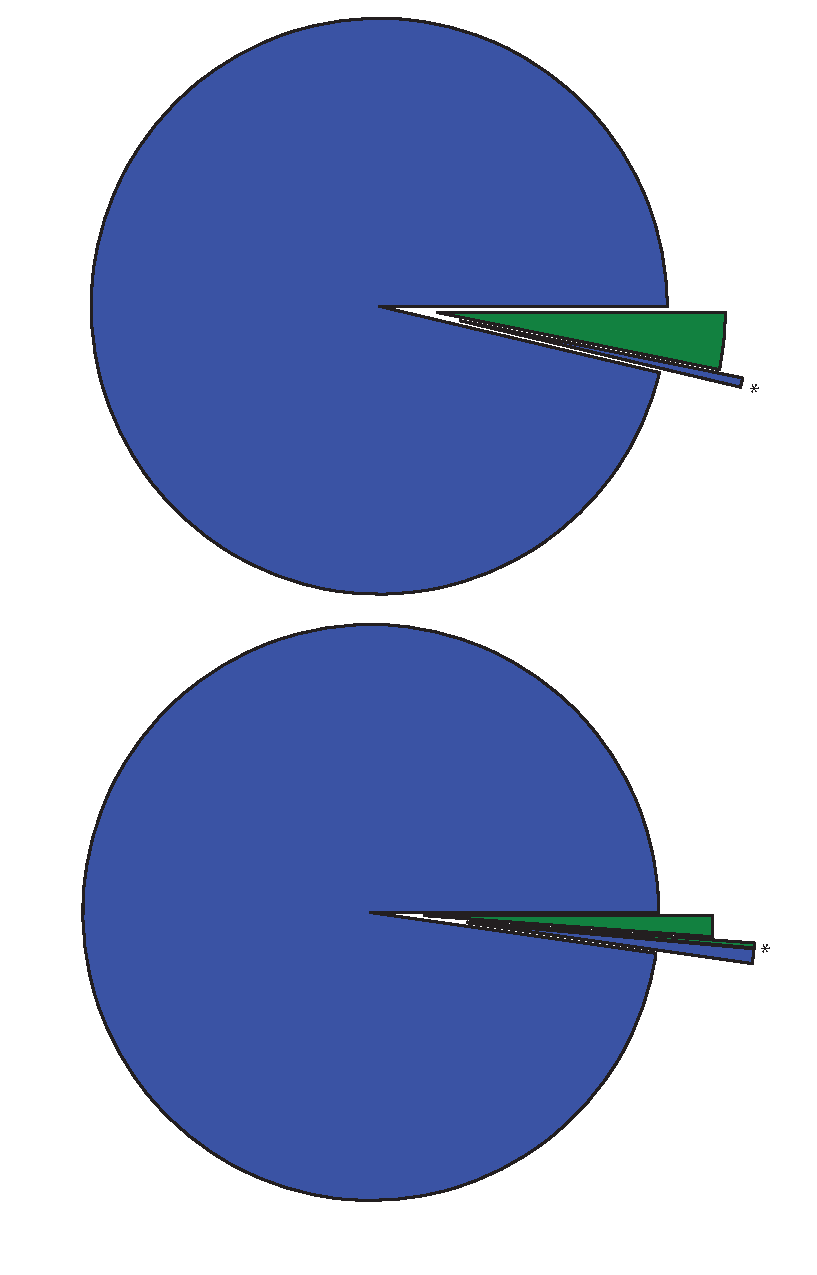
\includegraphics[width=\textwidth,height=\textheight,keepaspectratio]{./figures/ecolis-partitions.pdf}}
\caption{The fraction of partitions in spiked HMP datasets which contain single genomes (blue) and multiple genomes (green).  The section marked as * indicates partitions which contain spiked E. Coli reads which were subsequently assembled independently.  The top piechart is the single E. Coli spiked dataset and the bottom piechart is the multiple E. Coli spiked dataset.}
\label{ecolimap}
\end{figure}

\begin{figure}[h!]
\center{\includegraphics[width=\textwidth,height=\textheight,keepaspectratio]{./figures/ecoli-multi-genomes.png}}
\caption{The fraction of assembled contigs assembled from partitions containing spiked E. Coli reads associated with 0 to five of the E. Coli reference genomes.  The large majority of contigs contain reads associated with multiple genomes or to no genome.}
\label{fractionassembled}
\end{figure}

\begin{figure}[h!]
\center{\includegraphics[width=\textwidth,height=\textheight,keepaspectratio]{./figures/memory-requirements.png}}
\caption{Memory requirements to assemble subsets of Iowa corn soil metagenome}
\label{memory}
\end{figure}

\begin{figure}[h!]
\center{\includegraphics[width=\textwidth,height=\textheight,keepaspectratio]
{./figures/mockdiginormhist.pdf}}
\caption{  K-mer coverage of HMP mock community dataset before and after filtering approaches.}
\label{kmercoverage}
\end{figure}

\begin{figure}[h!]
\center{\includegraphics[width=\textwidth,height=\textheight,keepaspectratio]
{./figures/soildiginorm.pdf}}
\caption{K-mer coverage of Iowa corn and prairie metagenomes before and after filtering approaches.}
\label{diginormcoverage}
\end{figure}

\begin{figure}[h!]
\center{\includegraphics[width=\textwidth,height=\textheight,keepaspectratio]
{./figures/assembly-coverage.pdf}}
\caption{Coverage (median basepair) distribution of assembled contigs from soil metagenomes.}
\label{soilassemblycoverage}
\end{figure}

\begin{landscape}
\begin{table}[h!]
\center{\includegraphics[scale=0.8]{./figures/data-reduction.pdf}}
\caption{The total number of reads in original, filtered, and partitioned datasets and the computational resources required for filtering and partitioning.}
\label{datareduction}
\end{table}
\end{landscape}


\begin{landscape}
\begin{table}
\center{\includegraphics[scale=1.2]{./figures/assembly-stats.pdf}}
\caption{Assembly comparisons of unfiltered and filtered or filtered/partitioned datasets.  Assembly content similarity is based on the fraction of alignment of assemblies and similarly, the coverage of reference genomes is based on the alignment of assembled contigs to reference genomes.  Assembly summary statistics are also shown for multiple assemblers.}
\label{assemblystats}
\end{table}
\end{landscape}

\begin{landscape}
\begin{table}
\center{\includegraphics[scale=1.2]{./figures/mapping-summary-gpgc.pdf}}
\caption{Fraction of single-end (SE) and paired-end (PE) reads mapped to Iowa corn and prairie assemblies.}
\label{mappings}
\end{table}
\end{landscape}

\bibliography{assembly-paper}


\end{document}